
\documentclass[a4paper,12pt]{scrartcl}
\usepackage[utf8]{inputenc}
\usepackage{amsmath}
\usepackage{amsfonts}
\usepackage{listings}
\usepackage{float}
\usepackage[ngerman]{babel}
\usepackage{url}
\usepackage{enumerate}
\usepackage{graphicx}

\DeclareRobustCommand{\rchi}{{\mathpalette\irchi\relax}}
\newcommand{\irchi}[2]{\raisebox{\depth}{$#1\chi$}} 


%opening
\title{Statistik-Skript}
\author{Hans-Christian Heinz\\
hheinz@imn.htwk-leipzig.de\\
CC-BY-NC-SA}
\date{WS2013/14}
\setlength{\parindent}{0pt}

\begin{document}

\maketitle

\part{Wahrscheinlichkeitsrechnung}

\section{Wahrscheinlichkeiten}
\subsection{Zufällige Ereignisse}
Bedingungen für Experiment gegeben.\\
Versuch (Experiment): Realisierung der Bedingungen.\\
Ereignis: Ergebnis eines Experiments - soll beobachtet werden
\begin{itemize}
 \item heißt notwending wenn es zwingend eintritt
 \item heißt zufällig, wenn es eintreten kann oder nicht
\end{itemize}

\subsection{Relative Häufigkeiten, Wahrscheinlichkeitsbegriff}
$E$ - Menge von zufälligen Elementarereignissen\\
$e\in E$ - Menge von Bedingungen, die beim Versuch realisiert werden\\
Ereignis A: Teilmenge von $E$,$A\subseteq E$\\
\paragraph{Definition:} \textit{relative Häufigkeit}
\begin{description}
 \item[A,B] Ereignisse
 \item[n] Anzahl ausgeführter Experimente
 \item[k] Anzahl der Experimente bei denen A beobachtet wird
 \item[$\mathbf{A\cap B}$] das Ereignis, dass A und B beobachtet werden
 \item[$\mathbf{A\cup B}$] das Ereignis, dass A oder B beobachtet werden
 \item[relative Häufigkeit] $h_n(A) = \frac{k}{n}$
\end{description}

Eigenschaften von $h_n$
\begin{enumerate}
 \item $0\leq h_n(A)\leq 1$
 \item $h_n(E) = 1$
 \item Es sei $A\cap B = \emptyset$\\
 $$h_n(A\cup B) = h_n(A) + h_n(B) $$
\end{enumerate}

Für $n\rightarrow\infty$: $h_n(A)$ stabilisiert sich.

\begin{description}
 \item[W] Formalisierung nach Kolmogorow
 \item[MA] Sigma-Mengenalgebra von Teilmengen von $E$, d.h. $MA\subseteq 2^E =$ Menge aller Teilmengen von $E$\\
 und $E\in MA$
 $$A,B\in MA \rightarrow A\cup B \in MA \land A\setminus B\in MA$$
 $$\forall : A_i \in MA \rightarrow \bigcup^{\infty}_{i=1} A_i\in MA$$
\end{description}

$MA$ soll \glqq{}die interessierenden\grqq{} Ereignisse enthalten.\\
Bemerkung: $\bar{A}$ von $A$ und $A\cap B$ sind dann auch in MA\\
Beweis: $\bar{A} = E\setminus A, A\cap B = \overline{\bar{A}\cup\bar{B}}$
\\
Kolmogorow'sche Axiome (1933):
$P:\!MA\rightarrow R$ mit:
\begin{enumerate}
 \item $\forall A: A\in MA \rightarrow P(A) \geq 0 $
 \item $P(E) = 1$
 \item $\{A_i\}$ geg. $(A_i\in MA)$ mit $\forall i,j: i\neq j \rightarrow A_i \cap A_j = \emptyset$\\
 Dann $P(\bigcup^{\infty}_{i=1}A_i = \sum^{\infty}_{i=1}P(A_i)$
\end{enumerate}

\paragraph{Definition:} $[E,MA,P]$ heißt W-Raum\\

Beispiel:\\
$E = \{e_1,e_2,\dots,e_n\}$\\
$MA\subseteq 2^E = \{\underbrace{\{\},\{e_1\},\dots,\{e_n\},\{e_1,e_2\},\dots,\overbrace{\{e_1,\dots,e_n\}}^E}_{2^n Elemente}\}$\\
$p_1,p_2,\dots.p_n$ seien gegeben mit $\forall i: p_i\geq 0$ mit $\sum^{n}_{i=1}p_1 = 1$\\
\textbf{A} zufälliges Ereignis\\
$\hookrightarrow  P(A) = \sum_{i: e_i\in A} p_i$\\
\\
Wichtiger Spezialfall: Laplace'scher W-Raum\\
alle Versuchsausgänge gleichwertig, d.h. $\forall i: p_i = \frac{1}{n}$\\
$\hookrightarrow P(A) \frac{\text{Anzahl der } e_i\text{, die A bewirken}}{n}$\\
Mit diesen P heißt $[E,MA,P]$ Laplace'scher W-Raum.
\\
%KW42
\\
Wiederholung:
\paragraph{Ereignis und Elementarereignis} \quad\\
Ereignis: Ergebnis eines Experiments (im Modell: Menge von Elementarereignissen)\\ 
Elementarereignis: Satz von Bedingungen (im Modell: nicht näher bestimmt)
\paragraph{Warum Sigma-Mengenalgebra} Zur vollständigen Erfassung (mathematischen Modellierung) von Wahrscheinlichkeiten; um auch verm. uninteressante Ereignisse zu beinhalten; damit man z.B. das Ereignis \glqq{}nicht 3\grqq{} berechnen kann, indem man $1-p(3)$ bildet
\\
Vorlesung
\\
\subsection{Unabhängige Ereignisse} 
A,B (aus MA) heißen unabhängig, wenn $$P(A\cap B) = P(A) * P(B)$$.\\
A = \{Professer, 7:30, pünktlich zur Vorlesung\}\\
B = \{Morgen Milchreis in der Mensa\}\\
C = \{Morgen Gewitter\}\\
D = \{Stromausfall\}\\
$rightarrow$ nicht modellierbar/entscheidbar
Ein Ereignis ist immer stark abhängig von seinem Gegenteil!\\
Beispiel für Unabhängigkeit:\\
2 Würfel, A = \{Gerade Augenzahl\}, \{B = Augenzahl$\geq$2\}\\
\paragraph{Insgesamt unabhängige Ereignisse}\quad\\
Ereignis $A: \in MA \;(i=1,\dots,n)$ heißen insgesamt unabhängig, wenn für jede Indexmenge $\{i_1,\dots,i_k\}\subseteq \{1,\dots,b\}$ gilt: 
$$P(A_{i_1}\cap\dots\cap A_{i_k})=P(A_{i_1})*\dots *P(A_{i_k})$$
\paragraph{Definition:} $[E,MA,P]$ sei gegebener W-Raum\\
Es gelte $B\in MA$ und $P(B)>0$\\
Bedingte W von A unter Bedingung B:\\
$$P_B(A) = P(A|B) = \frac{P(A\cap B)}{P(B)}$$
Bemerkung: A,B unabhängig
$$\hookrightarrow P(A|B)=\frac{P(A\cap B)}{P(B)}\overset{!}{=}\frac{P(A)*P(B)}{P(B)}=P(A)$$
\paragraph{Satz:} $P(A|B)$ ist eine W, d.h. gibt
\begin{enumerate}[(a)]
 \item $\forall A\quad A\in MA \rightarrow P(A|B)>0$
 \item $P(E|B) = 1$
 \item $P(\bigcup^{\infty}_{i=1}A_i|B) = \sum_{i=1}^\infty P(A_i|B)$\\
	bei $\forall i,j \; j\neq i\rightarrow A_i \cap A_j \neq \emptyset $
\end{enumerate}

Beweis:
\begin{enumerate}[(a)]
 \item $A\cap B \in MA \rightarrow P(A\cap B)\geq 0 \rightarrow \frac{P(A\cap B)}{P(B)} \geq 0 $
 \item $P(E|B) = \frac{P(E\cap B}{P(B)} = \frac{P(B)}{P(B)} = 1$
 \item $P(\bigcup^{\infty}_{i=1}A_i|B) = \frac{P([\bigcup^{\infty}_{i=1}A_i]\cap B)}{P(B)} = \frac{P([\bigcup^{\infty}_{i=1}A_i\cap B])}{P(B)}$\\ alle $A_i\cap B$ sind \underline{durchschnittsfremd}\\
 $=\frac{\sum^\infty_{i=1}P(A_i\cap B}{P(B)} = \sum^\infty_{i=1}P(A_i|B)$
\end{enumerate}

\paragraph{Definition:} $[E,MA,P_B]$ heißt bedingter W-Raum

\subsection{Sätze zu bedingten Wahrscheinlichkeiten}
\begin{description}
 \item[Multiplikationssatz:]\quad\\ $A_1,\dots,A_n \in MA$\\
 Dann gilt
 $$P(\bigcap^\infty_{i=1}A_i) = P(A_1) * P(A_2|A_1) * \dots * P(A_n|\bigcap^\infty_{i=1} A_i) $$
 Beweis: n=2, dann vollständige Induktion\\
 Beispiel: Urnenmodell, Kugelnziehen ohne Zurücklegen\\
 Urne enthalte 2 weiße, 3 rote und 5 schwarze Kugeln\\
  $A_1 = \{\text{1. Kugel ist weiß}\}$\\
  $A_2 = \{\text{2. Kugel ist weiß}\}$\\
  $A_3 = \{\text{3. Kugel ist schwarz}\}$\\
  $P(A_1\cap A_2 \cap A_3)$\\
  $= P(A_1)*P(A_2|A_1)*P(A_3|A_1\cap A_2)$\\
  $=\frac{1}{5}*\frac{1}{9}*\frac{5}{8}=\frac{1}{72}$
\end{description}
  \paragraph{Definition:} Die (unendliche) Folge $\{A_i\}$ heißt vollständiges Ereignis, wenn
  $\forall i \; A_i\in MA$\\
  $\forall i \forall j \; i\neq j \rightarrow A_i\cap A_j = \emptyset$\\
  $\bigcup^\infty_{i=1}A_i = E$\\
  E wird vollständig durch die Folge $\{A_i\}$ beschrieben
\begin{description}
 \item[Satz von der totalen Wahrscheinlichkeit:]\quad\\
 $A\in MA$\\
 $\{B_i\}$ - vollständiges Ereignissystem $\forall i\;B\in MA; P(B_i)>0 $\\
 Dann gilt: $$P(A) = \sum_{i=1}^\infty P(A\cap B_i) = \sum_{i=1}^\infty P(A|B_i) * P(B_i)$$
\end{description}

Beweis:
$$A = A\cap E = A\cap (\bigcup^\infty_{i=1}B_i)$$
$B_i$ durchschnittsfremd\\
$\hookrightarrow (A\cap B_i$ auch durchschnittsfremd\\
Also:
$$P(A) = \sum^\infty_{i=1}P(A\cap B_i)$$
$$= \sum^\infty_{i=1}P(A|B_i)*P(B_i)$$
Bsp.: 3 Urnen $U_i$ mit schwarzen, roten, weißen Kugeln\\
$U_1$: 3s, 3r, 2w\quad P(Aus $U_1$ wird gezogen) = 0.3\\
$U_2$: 1s, 2r, 1w\quad P(Aus $U_2$ wird gezogen) = 0.2\\
$U_3$: 4s, 0r, 6w\quad P(Aus $U_3$ wird gezogen) = 0.5\\
Wie groß ist W, dass eine rote Kugel gezogen wird?\\
$$P(r) = P(r|U_1)*P(U_1) + P(r|U_2)*P(U_2)+P(r|U_3)*P(U3)$$
$$P(r) = \frac{3}{8}*0.3 + \frac{1}{2}*0.2 + \frac{0}{10}*0.5 = \frac{17}{80}$$

\begin{description}
 \item[Ursachensatz (Satz von Bayes)]\quad\\ 
 Voraussetzungen wie zuvor
 $$P(B_i|A) = \frac{P(B_i) * P(A|B_i)}{\sum^\infty_{j=1}P(A|B_j)*P(B_j)}\leftarrow \text{Nenner }=P(A)$$
\end{description}
Beweis:
$$P(B_i\cap A) = P(A\cap B_i) $$
$$P(B_i|A)*P(A) = P(A|B_i)*P(B_i)$$
$$P(B_i|A) = \frac{P(A|B_i)*P(B_i)}{P(A)}$$
Urnenbeispiel wie zuvor:
$$P(U_i|r)\text{zu berechnen}$$
$$P(U_1|r) = \frac{P(U_1)*P(r|U_1)}{P(r)} = \frac{0.3*\frac{3}{8}}{\frac{17}{80}}= \frac{9}{17}$$

\paragraph{Lösung Übungsaufgabe vom 18.10.2013} \quad\\
$$P(A_1\cap A_2) = \frac{9}{36}=\frac{1}{4}=\frac{1}{2}*\frac{1}{2}=P(A_1)*P(A_2)$$
$$P(A_1\cap A_3) = \frac{1}{36}=\frac{1}{2}*\frac{1}{18}=P(A_1)*P(A_3) $$
$$P(A_2\cap A_3)\text{ analog}$$
$$P(A_1\cap A_2 \cap A_3) = 0 \neq P(A_1)*P(A_2)*P(A_3)$$
Jeweils paarweise unabhängig, aber insgesamt nicht unabhängig

\section{Zufallsgrößen (Zg)}
\subsection{Grundlegende Definitionen}
Motivation:\\
X - Zg, d.h. ein Zahlenwert nach einem Experiment (noch zu präzisieren)\\
\\
Von Interesse: Ereignisse \\
$\{e: X(e)\leq x\} $\\
$\{e: a<X(e)< b\} $\\
\\
\paragraph{Definition:} Mengensystem $\{(-\infty,x]|x\in\mathbb{R}\}$ wird betrachtet\\
BM sei die hierdurch erzeugte Sigma-Mengenalgebra (kleinste Sigma-Mengenalgebra, die obiges Mengensystem enthält). Die Elemente von BM heißen Borel-Mengen.\\
\\
Beispiele von Borel-Mengen\\
$\{x:\;a<x\leq b\} = \{x:\;x\leq b\}\setminus \{x:\;x\leq a\} $\\
$\{b\}$, es sei $\{a_i\}$ monoton wachsend mit $\underset{i\rightarrow\infty}{\lim}a_i = b$\\
$\{b\} = \bigcap^\infty_{i=1}\{x:\; a_i<x\leq b\}$\\
$\{x:\;a<x\leq b\}\cup \{x: \; c<x\leq d\}$\\
\\
Zg:\\
$[E,MA,P]$ - W-Raum\\
R - Menge der reellen Zahlen\\
Es sei $B\in BM$\\
$X: E\rightarrow R$ mit $\{e: X(e)\in B\}\in MA$ \\
bzw. $X^{-1}(B) \in MA$\\
Dann heißt X eine Zg.\\
\\
Bemerkungen:\\
Die Abbildung X heißt dann [MA,BM] - messbar.\\
Die Messbarkeit von [E,MA,P] auf [R,BM] übertragen\\
Also: Eine Zufallsgröße ist eine borel-messbare Abbildung.\\

  \begin{figure}[h]
    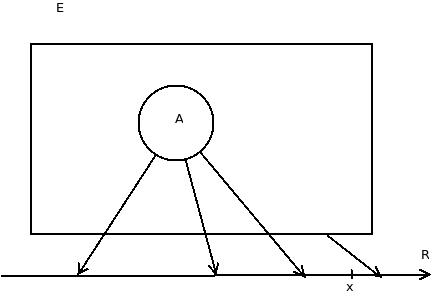
\includegraphics[scale=0.5]{./abbildungen/Borel.jpeg}
  \end{figure}

Verteilungsfunktion (Vf) zu einer Zg X:
$$F(x) = P(e:\;X(e)\leq x)$$
$$ \overset{kurz}{=} P(X\leq x)$$
Bemerkung: Wegen der Messbarkeit von X lässt sich zeigen, dass bei bel.$B\in BM$ gilt:\\
$$\{e\;X(e)\in B\}\in MA$$
Also existiert F(x).\\
Sprechweise: X ist verteilt nach F(x). Oder kurz: X $\sim$ F(x).\\
Es gilt immer
$$\underset{x\rightarrow-\infty}F(x) = 0$$
$$\underset{x\rightarrow\infty}F(x) = 1$$
F(x) ist monoton wachsend.\\

%KW 42 3

$F(x) = P(x\leq x)$ sei bekannt\\
$P(a<X\leq b)$ zu berechnen\\
$F(b) = P(e: X(e)\leq b)$\\
\quad$= P(\{e: X(e)\leq a\}\cup\{e: a<X(e)\leq b\})$\\
\quad$\underbrace{= P(X \leq a)}_{F(a)} + P(a<X\leq b)$\\
$\hookrightarrow P(a<X\leq b) = F(b) - F(a)$\\
\\
\paragraph{Definition:} Verteilungsfunktion F(x) gegeben, überall differenzierbar
$$f(x) = \frac{dF(x)}{dx}$$
heißt Dichtefunktion zur Zufallsgröße X.\\
$\hookrightarrow P(X\leq x) = \int_{-\infty}^{x}f(x) dx$\\
\\
\paragraph{Definition:} Zufallsgröße X,Y heißen mathematisch unabhängig, wenn
$$\forall x\forall y\;P(X\leq x \wedge Y\leq y) = P(X\leq x) * P(Y\leq y) $$
Bsp.: X,Y - Augenzahlen von 2 Würfeln\\
$Z = X+Y$, dann sind X und Z abhängig.\\
Körpergröße, Schuhgröße eines zufällig ausgewählten Menschen abhängig.\\
(Korrelation ist hinreichend, aber nicht notwendig!)\\
\\
Diskrete Zufallsgröße X: X kann nur Werte annehmen aus einer Folge $\{\dots,x_{-1},x_0,x_1,x_2,x_3,\dots\} $\\
\\
\paragraph{Satz:} Jede Verteilungsfunktion lässt sich in der Form
$$F(x) = a_1F_1(x) + a_2F_2(x)+a_3F_3(x)$$
darstellen, wobei
\begin{enumerate}[(a)]
 \item $a_i \geq 0,\;a_1+a_2+a_3=1 $
 \item $F_1(x)$ ist absolutstetig, d.h. es gibt eine Funktion f(x) mit
 $$F_1(x) = \int_{-\infty}^xf(y)dy \text{   (Lebesque Integral)}$$
 Riemann-Integral ist Spezialfall des Lebesque-Integrals\\
 d.h.
 $$F'(x) = f(x) \text{  fast überall} $$
 (abgesehen von einer Menge vom Lebesque-Maß 0)
 \item $F_2(x) $ eine diskrete Verteilungsfunktion it (reine Sprungfunktion)
 \item $F_3(x) $ singulär ist, d.h.\\
       $F'(x) = 0$ fast überall und stetig.
\end{enumerate}

\subsection{Das Stieltjes-Integral}

Motivation: Einf., um alle Verteilungsfunktionen einheitlich behandeln zu können. Verallgemeinerung des bekannten Riemann-Integrals.\\
Idee: Zu integrierende Funktion wird \glqq{}gewichtet\grqq{} integriert (nicht alle x-Werte sind gleich wichtig)\\
Gegeben seien Funktionen g(x) und F(x) und ein Intervall [a,b]. F(x) sei stetig in a, ansonsten rechtsstetig.\\
g(x) sei stetig.

\paragraph{Definition:} $\underbrace{Z(n,x)}_{\text{Vektor}(x_0\dots x_n)}$ sei eine Zerlegung von $[a,b]$\\
folgender Art::
$$a=x_0<x_1<x_2<\dots<x_n=b$$
Es sei
$$ \underbrace{V(n,x)}_{\text{abhängig von n und Vektor x}} = \sum^n_{i=1}|F(x_i)-F(x_{i-1})|$$
$$ V = \underset{Z(n,x)}{sup}\{V(n,x)\}=\text{kleinste obere Schranke bez. aller Zerlegungen von Z(n,x)}$$
V heißt totale Variation von F(x) in $[a,b]$\\
Bsp.:
$$F = \sin x \text{ in }[0,2\pi]$$
$$V=4$$
\paragraph{Definition:} des Riemann-Stieltjes-Integrals\\
Es sei
$$S(n,x) = \sum_{i=1}^n g(x_i) * |F(x_i) - F(x_{i-1})|$$
$$\lim_{n\rightarrow\infty} S(n,x) = \int^b_a g(x) dF(x) $$
\paragraph{Satz:} Grenzwert eindeutig bestimmt, unabhängig von Art der Zerlegung\\
\\
Uneigentliches Stieltjes-Integral
$$\int^\infty_{-\infty}g(x)dF(x) = \lim_{a\rightarrow-\infty}\lim_{b\rightarrow\infty}\int^{b}_{a}\dots $$
falls Grenzwert existiert.\\
\paragraph{Satz:} 
g(x) stetig und beschränkt auf $(-\infty,\infty)$\\
F(x) von beschränkten Totalvariation auf $(-\infty,\infty)$\\
$\hookrightarrow \int^{\infty}_{-\infty}\dots$ ex.\\
\\
Rechenregeln:
\begin{enumerate}[(a)]
 \item Es existiere $F'(x) = \frac{dF(x)}{dx}=f(x)$\\
 Denn $$\int^b_a g(x) dF(x) = \int^b_a g(x) \frac{dF(x)}{dx}dx $$
 $$=\int^b_a g(x)*f(x)dx $$
 \item $$\int^b_a[g_1(x)+g_2(x)]dF(x) = \int^b_a g_1(x)dF(x) + \int^b_a g_2(x) dF(x)$$
 \item $$\int^b_a g(x) d(F_1+F_2) = \int^b_a g(x) dF_1 + \int^b_a g(x) dF_2 $$
 \item $k_1, k_2$-Konst.
  $$\int^b_a [k_1*g]d[k_2*F] = k_1*k_2\int^b_a gdF $$
 \item $$\int^b_a gdF=\int^c_a\dots + \int^b_c\dots $$
 \item Partielle Integration $$\int^b_a g(x) dF(x) = g(b)*F(b)-\int^b_a F(x) dg(x) $$
\end{enumerate}
Ausblick\\
g(x) kann abzählbar unendlich viele Unstetigkeitsstellen haben, keine fällt mir einer Unstetigkeitsstelle von F(x) zusammen.\\
Zusammenfallen einiger Unstetigkeitsstellen $\rightarrow$ Lebesque-Stieltjes-Integral.

\subsection{Kennwerte von Zufallsgrößen}

X sei Zufallsgröße, $X\sim F(X)$\\
\paragraph{Erwartungswert:}
$$EX = \int^{\infty}_{-\infty} x dF(x) \overset{\text{Nur bei Ex. von f(x)}}{=} \int^{\infty}_{-\infty} x* f(x) dx$$
Interpolation: Mittelwert der Versuchsausgänge\\
Bsp.: Würfel Verteilungsfunktion F(x)

$$EX = \int^{\infty}_{-\infty} x dF(x) = 1*\frac{1}{6}+2*\frac{1}{6}+\dots+6*\frac{1}{6} = 3.5 $$
Andere Schreibweise
$$EX = \int^{\infty}_{-\infty} xdF(x) = \int_E X(e)dP(de) $$
Integration über die Menge der Elementarereignisse\\
Regel: $a,b \in \mathbb{R}: X,Y $ Zufallsgröße
$$E(a*X + b*Y) = a* EX + b*EY $$
\paragraph{Varianz:}
$$VarX = E(X-EX)^2$$
$$= E(X^2-2*X +EX +(EX^2))$$
$$= EX^2 - (EX)^2$$
$$= \int^{\infty}_{-\infty}(x-EX)^2 dF(x)$$
a sei Konstante
$$Var(a*X) = E(a*X - a*EX)^2 = a^2E(X-EX)^2=a^2*VarX$$

\paragraph{Streuung}
$$StrX = \sqrt{VarX} $$

Beispiel: $F(x) = 0 \text{ für } x\leq 0; x \text{ für } x\in (0,1]; 1 \text{ für } x>1$\\
EX, VarX berechnen

\paragraph{Linearer Zusammenhang von Zufallsgrößen}\quad\\
\begin{description}
 \item[Kovarianz:] $$Cov(X,Y) = E[(X-EX)*(Y-EY)]$$
 \begin{description}
  \item[Bemerkung 1:] $Cov(X,X)=Var(X) $
  \item[Bemerkung 2:] $Cov(X,Y)=E(X*Y)-EX*EY$
 \end{description}
 \item[Korrelation:]\quad\\
 \begin{description}
  \item[Idee: 1-Normierung]
    $$Korr(X,Y) = \frac{E[(X-EX)*(Y-EY)]}{\sqrt{E(X-EX)^2*E(Y-EY)^2}}$$
    Kovarianz im Zähler, Streuung im Nenner
  \item[Satz:] $-1\leq Korr(X,Y)\leq 1$
 \end{description}
\end{description}

Es gilt
$$Var(X+Y) = E(X+Y - EX-EY)^2$$
$$\; =E((X-EX)+(Y-EY))^2$$
$$\; =E[(X-EX)^2+2*(X-EX)*(Y-EY)+(Y-EY)^2]$$
$$\; =VarX + VarY + 2*Cov(X,Y)$$
X,Y unabhängig $\rightarrow Cov(X,Y)=0, Korr(X,Y)=0$\\
Umkehrung gilt im Allgemeinen nicht\\
Ausnahme: X,Y normalverteilt\\
\paragraph{Tschebyschew'sche Ungleichung}
$$P(|X-EX|\geq x * StrX) \leq \frac{1}{x^2}$$

\subsection{Beispiele für Verteilungsfunktion}
\begin{enumerate}[(a)]
 \item Diskrete Verteilungen \\
  \paragraph{Einpunkt-Verteilungen F(X)}\quad\\
  Es existiert Zahl a mit
  $$P(X=a) = 1 $$
  $$\int^a_{a-0}x dF(x) \underset{\text{Intergrand an Sprungstelle mal Sprunghöhe}}{=} a$$
  $$\int^a_{a-0} (x-a) dF(x) $$
  $$=(a-a)*1 = 0$$
  
 \paragraph{Gleichmäßige Verteilung}\quad\\
  n mögliche Versuchsausgänge $\{1,\dots,n\}$ alle gleichwahrscheinlich, d.h.
  $$P(X=k) = \frac{1}{n}\quad\quad k=1,\dots,n $$
  $$P(X\leq k) = \sum_{i=1}^k P(X=k)=\frac{k}{n} $$
  $$EX = \frac{n+1}{2}$$
  
  \paragraph{Binomialverteilung}\quad\\
  Ausgangspunkt: Benoulli'sches Schema\\
  A gegeben $(A\in MA)\quad p=P(A) > 0$\\
  X - Anzahl des Eintretens von A bei n unabhängigen Versuchen
  $$B(n,k) ) P(e:X=k) = \binom{n}{k} * p^k * (1-p)^{n-k} $$
  $$P(X\leq x) = \sum_{k:k\leq x} B(n,k) $$
  $$EX = n+p \quad\quad VarX = n*p*(1-p) $$
  
  \paragraph{Geometrische Verteilung}\quad\\
  $A \in MA$ - interessierendes Ereignis\\
  X - Anzahl von unabhängigen Versuchen bis erstmals A eintritt\\
  \{X=k\} bedeuetet: (k-1) Fehlversuche A im k-ten Versuch\\
  Geg.: $p=P(A)>0$\\
  $$P(X=k) = (1-p)^k * p\text{      mit }k=1,2,\dots$$
  $$\hookrightarrow EX = \frac{1}{p}\quad\quad VarX = \frac{1-p}{p^2}$$
  
  \item Stetige Verteilungen\\
  \paragraph{Gleichverteilung}\quad\\
  
  $$F(x) = P(X\leq x) = \left\{ 
  \begin{array}{l l l}
    0 & \quad \text{für $x\leq a$}\\
    \frac{x-a}{b-a} & \quad \text{für $x \in (a,b]$}\\
    1 & \quad \text{für $x>b $} 
  \end{array} \right. $$
  
  $$F'(x) = f(x) = \frac{1}{b-a} \text{ für } (a,b) $$
  
  $$EX = \frac{a+b}{2}\quad VarX=\frac{(b-a)^2}{12}$$
  Wichtiger Spezialfall: $a=0,b=1$\\
  
  \paragraph{Normalverteilung}\quad\\
  Zufallsgröße X heit normalverteilt mit Parametern $\mu$ und $\sigma$, wenn x folg. Dichte hat:
  $$nv(x,\mu,\sigma) = \frac{1}{\sigma * \sqrt{2*\pi}}* e^{-\frac{(x-\mu)^2}{2*\sigma^2}}$$
  $$\int^\infty_{-\infty}nv dx = 1$$
  $$NV(x,\mu,\sigma) = \int^x_{-\infty}nv(x,\mu,\sigma)dx $$
  $$EX = \mu \quad VarX = \sigma^2$$
  Wichtiger Spezialfall:
  $$\mu=0,\quad \sigma=1\quad \text{Standard-Normalverteilung} $$
  
  \paragraph{Student-Verteilung} (W.S. Gosset, engl. Statistiker, Pseudonym: Student)\\
  Vorbereitung: Gamma-Funktion (Euler 1730)
  $$\Gamma(x) = \int_0^{\infty}y^{x-1}*e^{-y}dy$$
  Bemerkenswert: Es gilt fü $x>1$ die Funktionalgleichung
  $$\Gamma(x) = (x-1)*\Gamma(x-1) $$
  $\Gamma(1) = 1$, $\Gamma(\frac{1}{2})=\sqrt{\pi}$\\
  Für natürliches x ist das die Fakultätsfunktion $(x-1)$!\\
  Dichte der Student-Verteilung für $x\in\mathbb{R}$ (mit n Freiheitsgraden)
  $$stu(x,n) = \frac{\Gamma(\frac{n+1}{2})}{\Gamma(\frac{n}{2})\sqrt{\pi *n}}*(1+\frac{x^2}{n})^{-\frac{n+1}{2}} $$
  symmetrisch bezüglich y-Achse\\
  $Stu(x.n) $ zugehörige Verteilungsfunktion\\
  \paragraph{Satz:} $\underset{n\rightarrow\infty}{\lim}Stu(x,n) = NV(x,0,1)$\\
  $X\sim Stu$\\
  $n\geq 2 \rightarrow EX=0$\quad\quad$n\geq 3 \rightarrow VarX = \frac{n}{n-2} $
  
  \paragraph{$\rchi^2$-Verteilung}\quad\\
  Dichte
  $$chiQ(x,n) = \left \{ 
  \begin{array}{l l}
    \frac{1}{2^{\frac{n}{2}}*\Gamma(\frac{n}{2})}*x^{\frac{n}{2}-1}*e^{-\frac{x}{2}} & \quad \text{, für }x>0\\
    0 & \quad \text{, für } x \leq 0
  \end{array} \right. $$
  
  Zugehörige Verteilungsfunktion ChiQ(x.n)\\
  Bem. Es gibt auch $\rchi$-Verteilungen. Falls X eine $\rchi$-Verteilung hat, hat $X^2$ eine $\rchi^2$-Verteilung
  
\end{enumerate}

\subsection{Simulation von Zufallsgrößen}
$F(x) = P(X\leq x)$ sei bekannt.\\
\\
Aufgabe: konkrete Stichprobe $x_1,\dots,x_n$ zu erzeugen (n unabhängige Experimente mit X)\\
Vorüberlegung:\\
Y sei auf $[0,1)$ gleichverteilte Zufallsgröße, d.h.
$$G(x) = P(Y\leq x) = x \text{   für }x\in[0,1)$$
\paragraph{Satz:} F(x) sei stetig und streng monoton wachsend. Dann gilt für die Zufallsgröße $F^{-1}(Y)$
$$P(F^{-1}(Y)\leq x) = F(x) $$
Beweis:
$$P(F^{-1}(Y)\leq x) = P(Y\leq F(x)) = F(x) $$
Realisierungen $y_i$ von Y sind per Zufallsgenerator erzeugbar\\
$F^{-1}(y_i)$ ist die i-te Realisierung von X.\\
Lösung obiger Aufgabe:\\
$y_i$ sei erzeugt
\begin{enumerate}[(a)]
 \item Setze $x_i = F^{-1}(y_i)$ falls die rechte Seite existiert und eine Zahl ist.
 \item Setze $x_i=a $, falls $F^{-1}(y_i)$ ein Intervall $[0,1)$ ist
 \item Setze $x_i=\min\{x: F(x) > y_i\}$, falls $F^{-1}(y_i)$ nicht existiert. 
\end{enumerate}

Beispiel: Würfel-Verteilungsfunktion
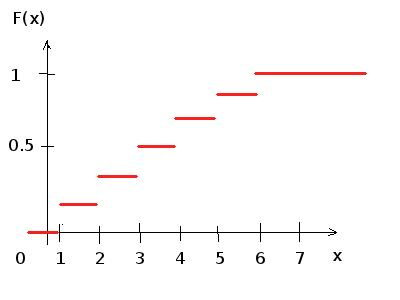
\includegraphics[scale =0.5 ] {./abbildungen/WurfelVerteilungsfunktion.jpg}

\begin{enumerate}[(a)]
\setcounter{enumi}{1}
 \item Es sei $y_i=0.5$\\
 $F^{-1}(y_i) = F^{-1}(0.5)=[3,4)$\\
 $\hookrightarrow x_i = 3 $
 
 \item Es sei $y_i = 0.51$\\
 $\min{x:F(x)>0.51}=4$
\end{enumerate}

 \subsection{Quantile}
 
 Zufallsgröße X, $x\sim F(x)$\\
 Es sei $0\leq p \leq 1$. Jede Zahle $Q_p$, die der Bedingung
 $$F(Q_p-0)\leq p \leq F(Q_p)$$
 genügt, heißt p-Quantil von F(x).\\
 0.5-Quantile heißen Mediane.\\
 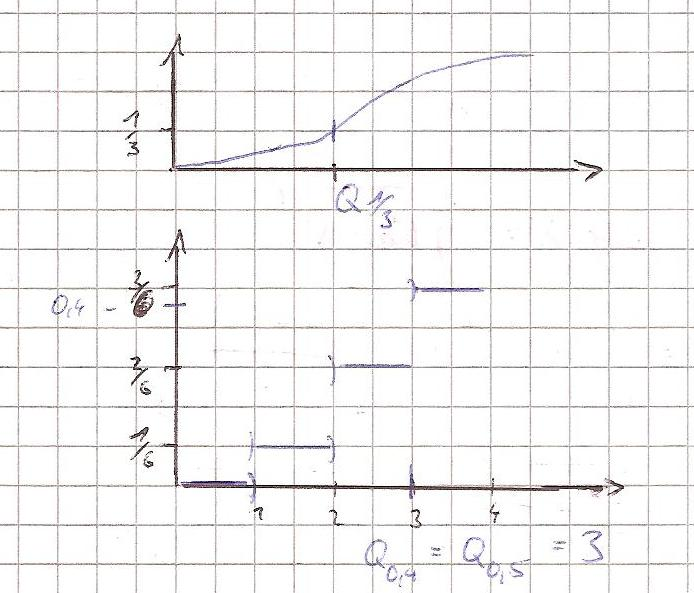
\includegraphics[scale=0.4]{./abbildungen/Quantile.jpg}\\
 Für Würfel-Verteilungsfunktion: 0.4-Quantil ist genau die 3, 0.45-Quantil auch.\\
 
 Jede Zahl aus $[3,4]$ ist Median, insbesondere auch die 4.\\
 Bemerkung: F(X) ist streng monoton $\rightarrow$ alle Quantile eindeutig.
 
 \section{Funktionen von Zufallsgrößen und Zufallsvektoren}
 
 \subsection{Funktionen einer einzelnen Zufallsgröße}
 
 Gegeben: W-Raum $[E,MA,P]$, Zg X, Funktion g(x)\\
 Bilde g(X). Laut Zufallsgrößen-Definition müsste g(X(e)) borel-messbar sein. X selbst ist borel-messbar. X bildet Ereignisse $A\in MA$ in Sigma-Mengenalgebra BM ab.\\
 \paragraph{Definition:} g(x) heißt borel-messbar, wenn für jedes $B\in BM$ gilt:
 $$g^{-1}(B)\in BM $$
 \paragraph{Satz:} Ist die Funktion g(x) stückweise stetig, dann ist sie borel-messbar.\\
 \\
 Beispiel: Quadrat einer Zufallsgröße\\
 X sei positive Zufallsgröße $X\sim F(x)$
 $$P(X^2\leq x) = P(X\leq \sqrt{x}) = F(\sqrt{x}) $$
 
 \subsection{Zufallsvektoren}
 Borel-Messbarkeit ist auf Funktionen mehrerer Variabler übertragbar.\\
 Folgende Funktionen sind borel-messbar:
 \begin{itemize}
  \item Vielfache
  \item Summen
  \item Produkte
  \item Quotienten (falls def.)
  \item Maximum, Minima
  \item Infikatorfunktionen
  \item Grenzwerte von Folgen einer Zufallsgröße
 \end{itemize}

 \paragraph{Definition:} $X_1,\dots,X_n$-Zufallsgröße über $[E,MA,P]$
 $$F(x_1,\dots,x_n) = P(X_1\,\dots,X_n\leq x_n)$$
 heißt gemeinsame Verteilungsfunktion der Zufallsgröße.\\
 Die $P(X_i\leq x_i)$ heißen Randverteilungen.\\
 \\
 F monoton wachsend bezüglich jedes x:\\
 $n=2$\quad\quad$P(X\leq x, Y\leq Y) \rightarrow P(X\leq x) = \lim_{y\rightarrow\infty}P(X\leq x, Y\leq y)$\\
 
 Berechnung von 
 $$P(a<X\leq b, c<Y\leq d)$$
 $$=\underbrace{F(b,d)-F(b,c)-F(a,d)+F(a,c)}_{\geq 0\text{ , sonst ist F keine Verteilungsfunktion}}$$
 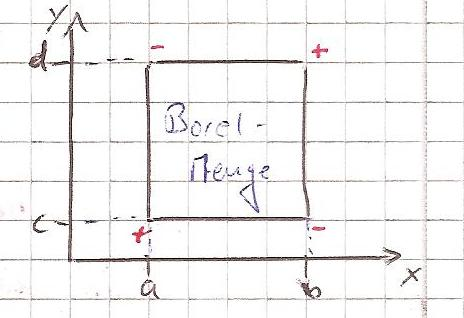
\includegraphics[scale = .5]{./abbildungen/borelmengen.jpg}\\
 
 \paragraph{Definition:}
 $$f(x_1,\dots,x_n) = \frac{\delta^nF(x_1,\dots,x_n)}{\delta x_1 \dots \delta x_n}$$
 heißt Dichtefunktion von $\begin{pmatrix}  X_1 \\  \vdots \\  X_n \end{pmatrix}$ , wenn die Ableitungen existieren und stetig sind (Voraussetzung des Satzes von Schwarz).\\
 \\
 \paragraph{Definition:} (Fall n=2, leicht verallgemeinerbar)\\
 Gegeben: Zufallsgrößen X,Y: $X\sim F_X(x)$  $Y\sim F_Y(x)$
 $$F_X(x|y) = P(X\leq x|Y=y) = \lim_{h\rightarrow 0} \frac{P(X\leq x, y-h<Y\leq y+h)}{P(y-h<Y\leq y+h}$$
 heißt bedingte Verteilungsfunktion von X unter der Bedingung Y=y, falls der Limes existiert.\\
 \paragraph{Definition:}
 $$E(X|Y=y) = \int_{-\infty}^\infty x dF_X(x)$$
 heißt bedingter Erwartungswert unter Bedingung Y=y, falls Integral existiert.\\
 Formeln für bedingte Dichten/bedingte Wahrscheinlichkeits-Verteilungen (diskreter Fall) $\rightarrow$ Literatur.\\
 \\
 \paragraph{n-dimensionale Normalverteilung:}\quad\\
 Zufallsvektor $X= \begin{pmatrix} X_1\\ \vdots\\ X_n \end{pmatrix}$ gegeben.\\
 $X_i$ nicht einpunktverteilt\\
 Erwartungsvektor $EX = \begin{pmatrix} EX_1\\ \vdots \\ EX_n \end{pmatrix}$ und die Kovarianzmatrix C seien bekannt.\\
 $$EX = \begin{pmatrix} EX_1\\ \vdots \\ EX_n \end{pmatrix} = \begin{pmatrix}\mu_1\\ \vdots\\ \mu_n \end{pmatrix}$$
 
 $$C=
 \begin{pmatrix} 
  Var(X_1) & Cov(X_1,X_2) & \dots & Cov(X_1,X_n) \\
  Cov(X_1,X_2) & Var(X_2) & \dots & Cov(X_2,X_n) \\
  \vdots & \vdots & \ddots & \vdots \\
  Cov(X_1,X_n) & \dots & \dots & Var(X_n) 
 \end{pmatrix} $$
 
 C ist symmetrisch und positiv definit $\rightarrow C^{-1}$ existiert\\
 \\
 X heißt normalverteilter Zufallsvektor, wenn er folgende Dichtefunktion hat:
 $$nv(x,\mu,X) = \frac{1}{\sqrt{(2\pi)^n * det(c)}}*e^{-\frac{(x-\mu)^T*C^{-1}*(x-\mu)}{2}}$$
 
 \subsection{Funktionen von Zufallsvektoren}
 Beispiel: Summe zweier Zufallsgrößen X und Y.\\
 $\{y_i\}$ sei eine Zerlegung der y-Achse
 $$\dots y_{-1}<y_{-1}<y_0<y_1<y_2<\dots$$
 $$P(X+Y\leq y) = \sum_{i=-\infty}^\infty P(X+Y|Y\in(y_i,y_{i+1}])*\overbrace{P(Y\in(y_i,y_{i+1}]}^{F_Y(y_{i+1})+F_Y(y_i)} $$
 Zerlegungsverfeinerung, Integral-Längen gegen 0:
 $$= \int^\infty_{-\infty} P(X\leq x-y | Y=y) dP(Y\leq y) $$
 falls X,Y unabhängig:
 $$= \int^\infty_{-\infty} F_X(x-y) dF_Y(y) $$
 Faltungsintegral $\overset{\text{falls Existenz der Dichten}}{\rightarrow} f_{x+y}(x) = \int^\infty_{-\infty} f_x(x-y)*f_y(y)dy$
 
 \section{Grenzwertsätze - die Brücke zur Statistik}
 
 \subsection{Konvergenzbegriffe für Folgen von Zufallsgrößen}
 
 W-Raum $[E,MA,P]$ gegeben; $X,Y,X_1,X_2,\dots$  - Zufallsgrößen\\
 E - sicheres Ereignis\\
 $\emptyset$ - unmögliches Ereignis: $P(\emptyset) = 0$\\
 $A\in MA$ heißt fast sicher, wenn $P(A) = 1$\\
 MA heißt fast unmöglich, wenn $P(A) = 0$\\
 X,Y heißen gleich, wenn $\forall e\quad e\in E\rightarrow X(e) = Y(e)$\\
 X,Y heißen fast sicher gleich, wenn $P(e:X(e) = Y(e))=1$\\
 Stochastische Konvergenz (auch "`Konvergenz in Wahrscheinlichkeit"'): Eine Folge $\{X_i\}$ von Zufallsgrößen konvergiert stochastisch gegen die Zufallsgröße X, wenn 
 $$\forall \epsilon_1 \forall \epsilon_2 \exists n_o(\epsilon_1,\epsilon_2) \forall n(\epsilon_1>0\wedge\epsilon_2>0\wedge n \geq n_o \rightarrow P(e: |X_n(e)-X(e)|\geq \epsilon_1)\leq \epsilon_2)$$
 kurz: $$\epsilon\quad\epsilon>0\rightarrow\lim_{n\rightarrow\infty}P(|X_n-X|\geq\epsilon)=0$$
 $$\{x_n\}^P\rightarrow X $$
 
 \paragraph{Fast sichere Konvergenz}
  
  $$P(e: \lim_{n\rightarrow\infty}X_n(e) = X(e)) = 1 $$
  kurz:
  $$\{X_n\}\overset{\text{f.s.}}{\rightarrow}X $$
  Interpretation:
  Es ist fast sicher, dasss für wachsendes n $X_n$ ein letztes Mal stark vor X abweicht (mehr als $\epsilon$), danach nie wieder.\\
  (Es ist im Grunde klassische Konvergenz für die meisten $\epsilon$ - aber eben nicht für alle.)\\
 \paragraph{Konvergenz im quadratischen Mittel}\quad\\
 $EX^2$ möge existieren
 $$\lim_{n\rightarrow\infty} E(X_n - X)^2 = 0$$
 Konvergiert den Verteilungen nach (schwache Konvergenz)
 $$X\sim F(x), X_n\sim F_n(x)$$
 $\{x_n\}$ konvergiert schwach gegen X, wenn
 $$\forall x (\text{F stetig an Stelle x})\rightarrow\lim_{n\rightarrow\infty}F_n(x)=F(x)$$
 \paragraph{Satz:}
 Fast sichere Konvergenz $\rightarrow$ stochastische Konvergenz\\
 stochastische Konvergenz $\rightarrow$ schwache Konvergenz
 
 \subsection{Gesetze der großen Zahlen}
 
 Zum Begriff\\
  $\{x_i\}$  - Folge von Zufallsgrößen. Es sei
  $$z_n = \frac{1}{n}\sum^{n}_{i=1} X_i$$
  Gegenstand ist das Konvergenzverhalten der Filge $\{z_n\}$\\
  \paragraph{Definition:} $\{x_i\}$ genügt den schwachen GGZ, wenn Konstante a existiert mit:
  $$\{z_n\}\overset{P}{\rightarrow}a$$
  \paragraph{Definition:} $\{x_i\}$ genügt den starken GGZ, wenn Konstante a existiert mit:
  $$\{z_n\}\overset{\text{f.s}}{\rightarrow}a$$
  Die GGZ sind Grundlage vieler Resultate der Statistik.\\
  Gefragt sind notwendige und hinreichende Bedingungen, insbesondere für starkes GGZ.\\
  Spezialfall:\\
  Alle $X_i$ insgesamt unabhängig und identisch verteilt. $\rightarrow$ wichtige Resultate bekannt.\\
  Relative Häufigkeit\\
  n - Anzahl von Experimenten\\
  k - Anzahl der Experimente, bei denen A beobachtet wurde\\
  $h_n(A)$ wird mit Hilfe von Zufallsgrößen definiert:
  $$X_i =  \left\{ \begin{array}{l l}
    0 & \quad \overline{A}\text{ im i-ten Versuch}\\
    1 & \quad A \text{ im i-ten Versuch}
  \end{array} \right. h_n(A) = \frac{\sum^n_{i=1}X_i}{n}$$
 
 Satz von Bernoulli (Jakob, 1654-1705)\\
 $\epsilon>0$ beliebig, p = P(A). Dann gilt
 $$\lim_{n\rightarrow\infty} P(|h_n(A)-p|<\epsilon)=1$$
 D.h. $\{h_n(A)\}\overset{P}{\rightarrow}p$ (stochastische Konvergenz)\\
 $\sim$ genügt dem schwachen GGZ.\\
 Satz von Borel(1909)
 $$\{h_n(A)\}\overset{\text{f.s.}}{p}$$
 Beweis mit Hilfe des Satzes von Kolmogorow
 $$\forall i\quad EX_i = P(A)*1 + (1-P(A))*0 = P(A) = p$$
 d.h. für alle Summanden in $h_n(A)$
 $$\hookrightarrow Eh_n(A) = \frac{n*p}{n} = p$$
 
 \subsection{Der Zentrale Grenzwertsatz (ZGS)}
 \paragraph{Definition:} Wenn eine Summe von Zufallsgrößen (z.B. arithmetische Mittel) asymptotisch normalverteilt ist, sagt man: "`Es gilt der ZGS"'. (Das ist in vielen Fällen so.)\\
 Satz von Lindeberg-Lévy\\
 $\{x_i\}$ - Folge von insgesamt unabhängigen, identisch verteilten Zufallsgrößen mit endlicher Varianz.\\
 Es sei
 $$Y_n = \sum_{i=1}^nX_i\text{  und  }\mu=EX_1\quad \sigma^2 = VarX_1 \neq 0$$
 Es gilt $EY_n = n*\mu$ und wegen der Unabhängigkeit $VarY_n = n*\sigma^2$\\
 Für die Zufallsgröße
 $$z_n = \frac{Y_n-n*\mu}{\sigma * \sqrt{n}} = \frac{\frac{Y_n}{n}-\mu}{\frac{\sigma}{\sqrt{n}}}$$
 $\frac{Y_n}{n}$ - arithmetisches Mittel\\
 $\mu$  - $E(\frac{Y_n}{n})$\\
 $\frac{\sigma}{\sqrt{n}} $ - $Str(\frac{Y_n}{n})$\\
 Mit der Verteilungsfunktion $F_n(x) = P(Z_n \leq x)$ gilt dann $EZ_n = 0$\\
 \paragraph{Satz von Lindeberg-Lévy:} Es gilt der ZGS, insbesondere
 $$\lim_{n\rightarrow\infty}F_n(x) = \int^x_{-\infty}nv(y,0,1)dy = \frac{1}{2*\pi}*\int^x_0e^{-\frac{y^2}{2}}dy $$
 Sprechweise: $\{Z_n\}$ ist asymptotisch normalverteilt.\\
 Zusatz:\\
 Existiert $E|X_i|^3$, ist die Konvergenz sogar gleichmäßig.\\
 Folgerung: n sei groß $\rightarrow P(a<Z_n\leq b) \approx \frac{1}{2*\pi}*\int^b_a e^{-\frac{y^2}{2}} dy$
 
  Bemerkung: $Y_n$ ist als Summe darstellbar. A sei interessierendes Ereignis mit $P(A) = p$. X sei folgende Zufallsgröße:
  $$X=\left\{ 
  \begin{array}{l l }
    1 & \quad \text{falls A eintritt}\\
    0 & \quad \text{sonst} 
  \end{array} \right. $$
  $\hookrightarrow EX=p, VarX = EX^2-(EX)^2$\\
  $=p-p^2=p(1-p)$\\
  Mit X werden n Versuche gemacht $\rightarrow x_1,\dots,x_n$\\
  Dann ist $Y_1 = \sum\limits^{n}_{1=i}X_i$\\
  \\
  Für die Zufallsgröße
  $$Z_n = \frac{\overbrace{Y_1-n*p}^{EY_n}}{\underbrace{\sqrt{n*p*(1-p)}}_{StrY_n}}$$
  gilt dann wieder $EZ_n = 0, VarZ_n = 1$.\\
  \paragraph{Satz von Moivre-Laplace:}\quad\\
  Die Zufallsgröße $Z_n$ sind asymptotisch standardnormalverteilt:
  $$\lim_{n\rightarrow \infty}P(Z_n\leq x) = NV(x,0,1)$$
  Für große n gilt
  $$P(a<Z_n\leq b) \approx \frac{1}{2\pi}\int^b_a e^{-\frac{y^2}{2}}dy $$
  $$=P(a*\sqrt{n*p*(1-p)}+n*p < Y_n \leq b*\sqrt{n*p*(1-p)}+n*p)$$
  Für ausreichend gute Näherungen sollte gelten
  $$n*p*(1-p)>9$$
  d.h.
  $$n>36\text{ bei }p=0.5$$
  
  Beispiel:\\
  Integralberechnung nach Monte-Carlo-Methode\\
  Motivation: Methode für zahlreiche best. Integrale anwendbar.\\
  Aufgabe:
  $$I=\int^\pi_0\sin x dx\quad(=2,\text{ Erg. bekannt})$$
  Ansatz: Der Kurvenverlauf wird in ein Rechteck eingehüllt.
  Fläche des Rechtecks $=\pi$.\\
  Es werden n über Rechteck gleichverteilte Punkte $(X_i,Y_i)$ in das Rechteck "`geworfen"'. Voraussetzung:\\ 
  \quad Versuche insgesamt unabhängig,\\
  \quad $\forall i:\quad X_i,Y_i\text{ unabhängig}$,\\
  \quad $X_i\sim [0,\pi]\text{ - Gleichverteilung}$\\
  \quad $Y_I\sim [0,1]\text{ - Gleichverteilung} $\\
  Es sei $A=\{e: Y_i\leq\sin(X_i)\}$
  $$p=P(A)=\int^\pi_0\int^{\sin x}_0\frac{1}{\pi}dydx=\frac{2}{\pi}=0.636620$$
  $a_n(A)$ - absolute Häufigkeit der Punkte, die nicht oberhalb des Graphen von sin x in $[0,\pi]$ liegen.\\
  $h_n(A) = \frac{a_n(A)}{n}$ - relative Häufigkeit
  p wird geschätzt durch $h_n(A)$.
  Beispiel-Daten:\\
  $n=1000$, davon\\
  $a_n(A)=6377$ Punkte oberhalb von $\sin x$\\
  $h_n(A)=0.6377$\\
  I wird geschätzt als Teilfläche 63.77\% der Gesamtfläche vom Rechteck der Größe $\pi$: $I\approx0.6377*\pi=2.000252$\\
  \\
  Problem: Abweichung des "`wahren"' p-Wertes von der zufälligen Realisierung $h_n(A)=0.6377$.\\
  Abschätzung der Genauigkeit\\
  Für die absolute Häufigkeit $a_n(A) = h_n(A)*n$ gilt nach dem Satz von Moivre-Laplace, dass
  $$Z_n = \frac{a_n(A)-n*p}{\sqrt{n*p*(1-p)}}=\frac{(h_n(A)-p)\sqrt{n}}{\sqrt{p*(1-p)}}$$
  asymptotisch normalverteilt ist.\\
  Für n=10000 liegt NV praktisch vor.\\
  \\
  Zufallsgröße $Z\sim NV(x,0,1);\quad t>0$ wird so bestimmt, dass
  $$P(-t<Z\leq t) = \frac{1}{\sqrt{2\pi}}\int^t_{-t}e^{-\frac{y^2}{2}}dy = 0.95$$
  Lösung: $t=1.96$ (geringfügig zu groß)\\
  Es gilt sogar $P(-1.96<Z\leq1.96)>0.95$\\
  $\underset{\text{n groß}}{\hookrightarrow} P(-1.96<Z_n\leq 1.96) >0.95$\\
  \\
  Frage 1: Wie genau wird p durch $h_n(A)$ approximiert?
  $$0.95<P(-t<Z_n\leq t)$$
  $$=P(|h_n(A)-p| \leq t*\frac{\sqrt{p(1-p)}}{\sqrt{n}})$$
  $$< P(|h_n(A)-p|\leq \frac{1}{2*\sqrt{n}}) \quad\quad|t=1.96$$
  $$= P(\sim \leq \frac{0.98}{\sqrt{n}})$$
  $$<P(|h_n-p|\leq \frac{1}{\sqrt{n}})$$
  Frage 2: Welche Werte kommen für p in Frage, so dass $-t<Z_n\leq t$ gilt?\\
  Dazu: Lösung der Gleichungen $Z_n = \pm t$ (für $a_n(A)=6377$)
  $$\frac{a_n(A)-n*p}{\sqrt{n*p*(1-p)}}=\pm t$$
  $$(a_n(A)-n*p)^2 = n*p*(1-p)*t^2$$
  $$\hookrightarrow p^2-\frac{2*a_n(A)+t^2}{n+t^2}*p + \frac{a_n(A)^2}{n^2+n*t^2} = 0$$
  $$p_1 = \frac{2*a_n(A)+t^2}{2*(n+t^2}\sqrt{\frac{2 a_n(A)+t^2}{2*(n+t^2}-\frac{a_n(A)^2}{n^2+n*t^2}}$$
  $$p_2 = \sim + \sim $$
  Einsetzen obiger Beispiel-Daten:\\
  $n=10000$\\
  $a_n(A) = 6377$\\
  $t = 1.96$\\
  $\hookrightarrow p_1 = 0.628228$\\
  $\hookrightarrow p_2 = 0.647066$\\
  Für p-Werte aus $[p_1,p_2]$ ist das Versuchsergebnis plausibel\\
  $\hookrightarrow 1.973636 = \pi *p_1 < \int^\pi_0\sin x dx \leq \pi *p_2 = 2.032817$\\
  verlässlich mit 0.95 Sicherheit.
 
 \subsection{Die empirische Verteilungsfunktion}
 
 Gegeben: die Zugfallsgröße $X\approx F(x)$, $F(x)$ stetig\\
 Ausführung von n insgesamt unabhängigen Versuchen mit X\\
 $\hookrightarrow X_1,\dots,X_n$\quad$X_i\approx F(x)$
 $$I(X_i,x)=\left\{\begin{array}{l l}
                  1 & \text{, wenn }X_i>x\\
                  0 & \text{ sonst}
                 \end{array}\right.
 $$
 
 Empirische Verteilungsfunktion zu F(x)
 $$Emp_n(x) = \frac{1}{n}\sum_{i=1}^n I(X_i,x)$$
 %Grafik fehlt
 \paragraph{Satz von Gliwenko} (Hauptsatz der mathematischen Statistik)\\
 $\epsilon > 0$ beliebig gegeben. Dann gilt für die Zufallsgrößen-Folge $\{D_n\}$ mit
 $$D_n = \underset{x\in\mathbb{R}}{sup}|Emp_n(x)-F(x)|$$
 $$P(\lim_{n\rightarrow\infty}D_n\leq\epsilon) = 1$$
 Bemerkung: Satz rechtfertigt, $Emp_n(x)$ als Ersatz für F(x) zu benutzen, falls F(x) unbekannt (n möglichst groß)\\
 \paragraph{Satz von Kolmogorow:}\quad\\
 Bei stetigem F(x) gilt:
 $$K(x) = \lim_{n\rightarrow\infty} P(\sqrt{n}*D_n\leq x) =
 \left\{\begin{array}{l l}
         0 & \text{ für } x\leq 0\\
         1+2*\sum_{i=1}^\infty(-1)^i*e^{-2i^2x^2} & \text{ für } x>0
        \end{array}\right.
$$

Bemerkung: Satz ist theoretische Grundlage für Kolmogorow-Anpassungstest
 
 \part{Statistik}
 \setcounter{section}{0}
 
\section{Grundlegende Begriffe der Statistik}

Gegenstand: Wahrscheinlichkeits-Aussagen
\begin{itemize}
 \item ohne Kenntnisse der Verteilungsfunktion
 \item mit Kenntnissen von Stichproben
\end{itemize}

Grundgesamtheit:\\
Gegeben: \begin{itemize}
          \item W-Raum $[E,MA,P]$
          \item der messbare Raum $[R,BM]$
          \item Zufallsgröße X: $E\rightarrow R$
          \item $F_X(x) = P(e:X(e)\leq x) $
          \item W-Raum $[R,BM,F_X(x)]$
         \end{itemize}
         
  $[R,BM,F_X]$ heißt Grundgesamtheit mit Verteilung $F_X$\\
  
  X - Zufallsgröße, $F_X(x)$ unbekannt (im Allgemeinen)\\
  n unabhängige Experimente mit X liefern Realisierungen $x_1,\dots,x_n$\\
  $\begin{pmatrix}
    x_1\\
    \vdots\\
    x_n
   \end{pmatrix}$ heißt konkrete Stichprobe von X aus der Grundgesamtheit\\
   $X_1,\dots,X_n$ - insgesamt unabhängige Zufallsgrößen mit Verteilungsfunktion $F_X(x)$ (Vorstellung: n gedachte Experimente)\\
   $\begin{pmatrix}
     X_1\\\vdots\\X_n
    \end{pmatrix}$ heißt mathematische Stichprobe\\
    \paragraph{Beschreibende Statistik:}\quad\\
    Wiedergabe vorhandener Daten durch Auswahl und geeignete Darstellung mit Bestimmung interessierender Kenngrößen\\
    (Diagramme, Häufigkeitstabellen, Mittelwerte,$\dots$)
    \paragraph{Schließende Statistik:}\quad\\
    Mathematische Auswertung gezielt erhobener Stichproben, Rückschlüsse auf die Grundgesamtheit\\
    \paragraph{Typische Aufgabenstellungen}\quad\\
    Punktschätzungen:
    \begin{itemize}
     \item W
     \item EX
     \item StrX, VarX
     \item Parameter von F(x)
     \item $\dots$
    \end{itemize}
  Aussagen über Verlässlichkeit\\
  Berechnung von Irrtumswahrscheinlichkeiten\\
  \\
  Intervallschätzungen:\\
  Schätzung eines Intervalls in das die Punktschätzung fällt mit Wahrscheinlichkeit, dass das auch geschieht.\\
  \\
  Hypothesentests:\\
  Ist Stichprobe mit Hypothese über Grundgesamtheit verträglich?\\
  \\
  Stichproben-Funktion:\\
  ist eine borel-messbare Funktion $g(x_1,\dots,x_n)$\\
  $\hookrightarrow(X_1,\dots,X_n)$ ist dann Zufallsgröße
  
  \section{Schätztheorie}
  \subsection{Punktschätzungen - grundlegende Definitionen}
  Zwei einführende Beispiele: Zufallsgröße $X \sim \underset{\text{i.A. unbekannt}}{F(x)}$ gegeben\\
  EX wird geschätzt durch die Zugfallsgröße
  $$M_n ) \frac{1}{n}\sum_{i=1}^n X_i $$
  $X_i$: Ergebnis von n Experimenten mit X\\
  Einsetzen einer konkreten Stichprobe 
  $\begin{pmatrix}
    x_1\\
  \vdots\\
  x_n
   \end{pmatrix}$\\
  $$\hookrightarrow m_n = \frac{1}{n} \sum_{i=1}^n x_i \approx EX$$
  VarX wird geschätzt durch
  $$V_n = \frac{1}{n-1}\sum_{i=1}^n \underset{\text{empirische Varianz}}{(X_i -M_n)^2} $$
  $v_n$ - Realisierung von $V_n$:
  $$v_n = \frac{1}{n-1}(x_i-m_n)^2 \approx VarX $$
  Interessant: Untersuchung der Verteilungsfunktion von $M_n$ und $V_n$\\
  Bemerkung: $M_n\sim F^{n*}(n*x)$\\
  $F^{n*}$ ist n-fache Faltung von F(x) mit sich selbst.\\
  P(A) wird geschätzt durhc $\underset{\text{Spezialfall von $m_n$}}{h_n(A)}$\\
  \\
  Verallgemeinerung\\
  t sei ein unbekannter Parameter der Verteilungsfunktion $F_X(x)$, also $t=t(F_X)$\\
  t sei zu schätzen: $t\in D$ (Wertebereich)\\
  Bemerkung: t kann ein Vektor sein\\
  Die Menge der in Frage kommenden Verteilungsfunktionen kann eingeschränkt sein (Beispiel: "`Familie"' der Normalverteilungen; $t=\binom{\mu}{\sigma})$\\
  Häufige Voraussetzungen:\\
  $X_1,\dots,X_n$ - insgesamt unabhängig Exemplare von X\\
  $(x_1,\dots,x_n)^T$ - konkrete Stichprobe\\
  g - borel-messbare Funktion: n-stellig\\
  Die Stichprobenfunktion $g(X_1,\dots,X_n)$ heißt Schätzfunktion bzw. \underline{eine} Punktschätzung für ("`den Punkt"') t.\\
  \\
  $g(x_1,\dots,x_n)$ wird als Ersatz für t benutzt.\\
  Aber mit welchem Grund?\\
  g sollte wünschenswerte Eigenschaften haben:
  \begin{description}
   \item[Erwartungstreue:] g heißt erwartungstreu, wenn
   $$\forall F_X\quad Eg(X_1,\dots,X_n) = t(F_X)\quad\text{ mit } \forall i\, X_i\sim F_x$$
   Eine Folge$\{g_n\}$ von Schätzfunktionen heißt asymptotisch erwartungstreu, wenn
   $$\forall F_X \lim_{n\rightarrow\infty}Eg_n = t(F_X)$$
   Systematischer Fehler (Synonyme: Verzerrung, Bias)
   $$Eg(X_1,\dots,X_n) - t(F_X)\text{ (i.a. ein Vektor)} $$
   Meist systematischer Fehler von g gegenüber t.\
   Bemerkung; Erwartungstreue Schätzfunktionen sind biasfrei
   \item[Konsistenz:] $\{g_n\}$ heißt schwach/stark konsistent, wenn $\{g_n\}\overset{\text{P/f.s.}}{\rightarrow}t(F_X)$\\
   Bessere Schätzfunktion\\
   $g_1$ heißt besser als $g_2$, wenn für alle $\epsilon>0$ und alle $t\in D$ gilt:
   $$P(|g_1(X_1,\dots,X_n)-t|\leq \epsilon)>P(|g_2(\dots)-t|\leq \epsilon) $$
   Wirksamere Schätzfunktion:\\
   $g_1,g_2$ - erwartungstreu bezüglich t\\
   $g_1$ heißt wirksamer als $g_2$, wenn für $t\in D$
   $$Var[g_1(X_1,\dots,X_n)]<Var[g_2(X_1,\dots,X_n)]$$
   Wirksamste Funktion $\dots$
  \end{description}
  
  \subsection{Punktschätzungen  - wichtige Sätze}
  
  \paragraph{Satz:} Hinreichend für schwache Konsistenz sind
  \begin{itemize}
   \item asymptotische Erwartungstreue
   \item $\lim_{n\rightarrow\infty}Var[g_n(X_1,\dots,X_n)]=0$
  \end{itemize}
  \paragraph{Satz:} $M_n$ ust erwartungstreu für EX. Beweis trivial.\\
  \paragraph{Satz:} X, $X_i\sim F(X)\quad X_i$ insgesamt unabhängig
  $$V_n = \frac{1}{n-1}\sum_{i=1}^n(X_i-M_n)^2\quad S_n=\sqrt{V_n}(\approx StrX)$$
  Behauptung: $V_n$ schätzt VarX erwartungstreu.\\
  Beweis: Zuerst Umschreiben von $V_n$ - Klammern ausmultiplizieren
  $$V_n =\frac{1}{n-1}\sum_{i=1}^n(X_i^2-2*X_i*M_n+M_n^2)$$
  $$V_n =\frac{1}{n-1}\sum_{i=1}^nX_i^2+\frac{1}{n-1}(-2*M_n*\sum_{i=1}^nX_i + \sum_{i=1}^n M_n^2)$$
  $$V_n =\frac{1}{n-1}\sum_{i=1}^nX_i^2+\frac{1}{n-1}(-2*M_n*n*M_n+n*M_n^2) $$
  $$V_n =\frac{1}{n-1}\sum_{i=1}^nX_i^2-\frac{n}{n-1}M_n^2$$
  Erwartungswertbildung ($X_i$ durch X ersetzbar, $\sum$ entfällt)
  $$EV_n = \frac{n}{n-1}(EX^2-EM_n^2) $$
 
  \paragraph{Hier fehlt ein Stück!}\quad \\
  
  Damit folgt:
  $$EV_n = \frac{n}{n-1}*[E(X^2)-\frac{1}{n}E(X^2)-\frac{n-1}{n}(EX)^2]$$
  $$=\frac{n}{n-1}*(\frac{n-1}{n}E(X^2)-\frac{n-1}{n}(EX)^2)$$
  $$=EX^2-(EX)^2=VarX$$
  
  Bemerkungen
  \begin{enumerate}[(a)]
   \item Wäre EX bekannt, könnte VarX durch
   $$W_n = \frac{1}{n}\sum_{i=1}^n(X_i-EX)^2 $$
   erwartungstreu geschätzt werden
   \item Mit
   $$V_n = \frac{1}{n}\sum^n_{i=1}(X_i-M_n)^2$$
   Wird VarX nur asymptotisch erwartungstreu geschätzt
  \end{enumerate}

  Weitere Resultate für den Fall $X\approx NV(x,\mu,\sigma)$\\
  $\hookrightarrow M_n\approx NV(x,\mu,\frac{\sigma}{n})$\\
  $\hookrightarrow V_n$ asymptotisch normalverteilt\\
  $\hookrightarrow M_n$ und $V_n$ sind unabhängig
  Es sei $S_n = \sqrt{V_n}$\\
  $\hookrightarrow T_n = \frac{M_n-\mu}{S_n} * \sqrt{n} \approx Stu(x,n-1)$\\
  $\hookrightarrow \frac{n-1*S^2_n}{\sigma^2}\approx ChiQ(x,n-1)$\\
  
  \paragraph{Schätzung einer Kovarianz}\quad\\
  Kovarianz zweier Zufallsgrößen X und Y
  $$Cov(X,Y) = E((X-EX)*(Y-EY))$$
  $((x_1,y_1),\dots,(x_n,y_n))$ sei konkrete Stichprobe zu (X,Y)\\
  Schätzwert für Cov:  $x=\begin{pmatrix}x_1\\\vdots\\x_n\end{pmatrix}\quad y=\begin{pmatrix}y_1\\\vdots\\y_n\end{pmatrix}$\\
  $$cov(X,Y) = \frac{1}{n}\sum_{i=1}^n[(x_i-\underbrace{m_n(x)}_{\text{emp Mittel zu x}})*(y_i-m_n(y))]$$
  Schätzung der Korrelation
  $$korr(x,y) = \frac{cov(x,y)}{\sqrt{\sum_{i=1}^n(x_i-m_n(x))^2*\sum_{i=1}^n(y_i-m_n(y))^2}} $$
  Schätzung einer Kovarianzmatrix zu einem Zufallsvektor $\begin{pmatrix}x_1\\\vdots\\x_n\end{pmatrix}$:\\
  Voraussetzung: hohe Anzahl von Realisierungen\\
  Ergebnis: $\begin{pmatrix}
		cov(x_1,x_1)& cov(x_1,x_2) & \dots & cov(x_1,x_n)\\
		\dots \\
		cov(x_1,x_n) & \dots & & cov(x_n,x_n)
	      \end{pmatrix}$
  Vorraussetzung: Stichprobenumfang $>>$ Dimension des Zufallsvektors
 
  \subsection{Intervallschätzungen}
    
  Synonym: Bereichs-Schätzungen\\
  Aufgabenstellung: Berechnung von P(|Parameterwert-Schätzwert|$\in$Intervall)\\
  \underline{Wichtige} Voraussetzung (für die folgende Aufgabe)\\
  $X\approx NV(x,\mu,\sigma)$\\
  $(X_1,\dots,X_n)$ sei mathematische Stichprobe zu X\\
  \paragraph{Aufgabe 1:}\quad\\
		$\mu = EX$ unbekannt und zu schätzen\\
		$\sigma^2 = VarX$ bekannt\\
  
  $M_n = \frac{1}{n}\sum_{i=1}^nX_i\approx NV(x,\mu,\frac{\sigma}{\sqrt{n}}$\\
  Nach ZGS gilt:
  $$0.95 = P(-1.96<\frac{M_n-\mu}{\frac{\sigma}{\sqrt{n}}}\leq 1.96)$$
  $$=P(M_n-\frac{1.96}{\sqrt{n}}*\sigma<\mu\leq M_n+\frac{1.96}{\sqrt{n}*\sigma)} $$
  $M_n$ ist Zufallsgröße $\to$ zufällige Intervallgrenzen\\
  Interpretation:\\
    Man kann mit W von 0.95 (Konfidenzniveau) darauf vertrauen, dass $\mu$ im angegebenen Intervall liegt.\\
    Das gilt für jede Realisierung $m_n$ von $M_n$.
  Also:
    Man berechne die \underline{Intervallgrenzen} (mit $m_n$ statt $M_n$)\\
    $\mu$ liegt dann im Intervall mti W 0.95\\
  Bemerkung:
  \begin{enumerate}[(a)]
   \item Falls X nicht normalverteilt ist, ist $M_n$ dennoch asymptotisch normalverteilt
   \item Ist $\sigma$ nicht bekannt, kann (notfalls) $V_n$ verwendet werden
  \end{enumerate}

  \paragraph{Aufgabe 2:}\quad\\
  wie Aufgabe 1, aber jetzt sei $\sigma$ unbekannt\\
  Nitzung der Student'schen T-Funktion
  $$V_n' = \frac{1}{n}\sum_{i=1}^n(X_i-M_n)^2\quad S'_n=\sqrt{V_n^2}$$
  $$T_n = \frac{M_n-\mu}{S_n'}*\sqrt{n-1}$$
  \paragraph{Satz:} $T_n\approx Stu(x,n-1)$\\
  Konstruktion von Intervallgrenzen $T_l,T_r$\\
  Vorgabe eines Konfidenzniveaus $\alpha$ (meist 0.95)\\
  Bestimmung von $t'$ si, dass $P(-t'<T_n\leq t') = \alpha$\\
  Berechnung der Zufallsgrößen
  $$T_l = -\frac{s_n'*t'}{\sqrt{n-1}}+M_n\quad T_r=\frac{s_n'*t'}{\sqrt{n-1}}+M_n $$
  Dann gilt
  $$\alpha = 0.95 = P(-t'<T\leq t') $$
  $$P(-t'< \frac{M_n-\mu}{s'_n}*\sqrt{n-1} \leq t' $$
  $$P(-\frac{s'_n*t'}{\sqrt{n-1}}+M_n<\mu \leq \frac{s'_n*t'}{\sqrt{n-1}}*M_n)$$
  $$=P(T_l<\mu\leq T_r) $$
  Einsetzung konkreter Realisierung $x_i$ für $X_i \to$ konkrete Intervallgrenzen
  
  \paragraph{Aufgabe 3:}\quad\\
  2-seitiges Konfidenzintervall für $\sigma$ gesucht
  Es sei $\mu = EX$ unbekannt
  $$V_n = \frac{1}{n-1}\sum_{i=1}^n(X_i-\underbrace{M_n}_{\text{emp. Mittelwert}})^2 $$
  $$\chi^2 = \frac{n-1}{\sigma^2}*V_n^2 = \frac{1}{\sigma^2}*\sum_{i=1}^n(X_i-M_n)^2 $$
  \paragraph{Satz:}
  $$\chi^2\approx ChiQ(x,n)$$
  Vergabe eines Konfidenzniveaus $\alpha$ (meist 0.95)\\
  Bestimmung von $t_l$, so dass $P(\chi^2\leq t_l) = \frac{\alpha}{2}$\\
  Bestimmung von $t_r$, so dass $P(\chi^2 > t_l) = \frac{\alpha}{2}$\\
  $\hookrightarrow P(t_l<\chi^2\leq t_r) = \alpha$
  %Bild fehlt: ChiQ-Verteilung
  Zum testen sei Hypothese $H:\sigma = \sigma_0$
  \begin{enumerate}[(a)]
   \item Einsetzen von $\sigma_0$ in $\chi^2$-Formel
   \item $t_l,t_r$ berechnen
   \item Konkrete Stichprobe in $\chi^2$-Formel einsetzen - Konkreter $\chi^2$-Wert!\\
  \end{enumerate}
    $$\text{Test: }\chi^2\in(t_l,t_r]?$$\\
    \begin{itemize}
      \item wenn ja: Es gibt keinen Grund, H abzulehnen.
      \item wenn nein: H ist abzulehnen, weil bei Richtigkeit ein unwahrscheinliches Ereignis mit W $1-\alpha$ eingetreten wäre, was unglaubhaft ist.
    \end{itemize}
   P(Fehler 1. Art) = P(Ablehnung zu Unrecht) = $1-\alpha$\\
   P(Fehler 2. Art) = P(Nicht-Ablehnung zu Unrecht) = keine Aussage möglich (ohne weiteres
   
  \paragraph{Aufgabe 4:} wie Aufgabe 3, aber $\mu = EX$ bekannt\\
  $V_n'$ in $\chi^2$-Formel verwenden (Dividieren durch n, $\mu$ statt $M_n$)\\
  ChiQ(x,n-1) verwenden\\
  Ansonsten analog vorgehen
  
  
  \subsection{Maximum-Likelihood-Schätzmethode}
  
  $\begin{pmatrix}
    x_1\\\vdots\\x_n
   \end{pmatrix}$ - konkrete Stichprobe aus Grundgesamtheit
   $$[R,BM,F_X(x,t)]$$
   $$t=\begin{pmatrix}
    t_1\\\vdots\\t_n
   \end{pmatrix} \text{ unbekannter Punktvektor, }t\in D\text{ möglicherweise bekannter Bereich}$$
   \begin{enumerate}[(a)]
    \item X hat diskrete Verteilung; k Werte möglich: $a_1,dots,a_k$; $p_i=P(X=a_i)$\\
    $p_i(a_i,t_1,\dots,t_n)$ - Funktion des Vektors t\\
    Likelihood-Funktion: $$L(x_1,\dots,x_n,t_1,\dots,t_m) = \prod_{i=1}^n p_i(x_i,t_1,\dots,t_m)$$
    \item Stetiger Fall\\
    $F_X(x,t)$ sei nach x differenzierbar $\to f(x)=\frac{d(F_X(x,t)}{dx}$\\
    Likelihood-Funktion:
    $$L(x_1,\dots,x_n,t_1,\dots,t_m) = \prod_{i=1}^n f(x_i,t_1,\dots,t_m)$$
   \end{enumerate}
 ML-Methode zum Finden einer Punktabschätzung für t\\
 Vorschrift: \underline{Der} Punkt $t*$ wird als Schätzwert verwendet, für den die Likelihood-Funktion bei vorliegender Stichprobe x maximal wird.\\
 formal: $L(x,t*) = \underbrace{\max_{t\in D}L(x,t)}_{\text{Existenz, Eindeutigkeit nicht sicher}}$\\
 Mögliche Methoden $t*$ zu finden:\\
 L nach allen $t_i$ differenzieren, Ableitung $= 0$ setzen\\
 $\hookrightarrow$ Gleichungssystem (m Gleichungen) lösen\\
 besser: ln(L) ableiten\\
 $\hookrightarrow ln(\prod\dots)$ ist eine Summe\\
 Bemerkung: Unter bestimmten Bedingungen ist eine ML-Schätzung
 \begin{itemize}
  \item erwartungstreu
  \item konsistent
  \item asymptotisch normalverteilt
  \item asymptotisch effektiv
  \item erschöpfend
 \end{itemize}
 
 ML-Schätzung einer Streuung\\
 $X\approx NV(x,0,\sigma)$ mit $\mu=0$ und $\sigma$ unbekannt\\
 $\begin{pmatrix}
   x_1\\x_2
  \end{pmatrix}$ sei konkrete Stichprobe vom Umfang $n\geq 2$ mit $x_1=-2,x_2=1$\\
  $\sigma$ ist mit ML-Methode zu schätzen
  $$L(-2,1,\sigma) = \frac{1}{2\pi\sigma^2}*e^{-\frac{-2*-2}{2\sigma^2}}*e^{-\frac{1*1}{2\sigma^2}}$$
  $$= \frac{1}{2\pi\sigma^2}*e^{-\frac{5}{2\sigma^2}} $$
  $$L'(-2,1,\sigma) = \frac{-2}{2\pi\sigma^3}*e^{-\frac{5}{2\sigma^2}} +\frac{1}{2\pi\sigma^2}*\frac{2*5}{2\pi\sigma^3}*e^{-\frac{5}{2\sigma^2}}$$
  $$=\frac{-1}{\pi\sigma^3}*e^{\dots}+\frac{5}{2\pi\sigma^5}*e^{\dots} \overset{!}{=}0$$
  $$\hookrightarrow 2\sigma^2=5$$
  $$\hookrightarrow \sigma = \sqrt{\frac{5}{2}}$$
  $L''$ wäre zu untersuchen für den Maximumsnachweis\\
  Kürzer: $\epsilon$ klein, $L'$ programmieren (Matlab)
  $$L'(2,1,\sqrt{\frac{5}{2}}-\epsilon)<0$$
  $$L'(2,1,\sqrt{\frac{5}{2}})=0$$
  $$L'(2,1,\sqrt{\frac{5}{2}}+\epsilon)>0$$
  $\to L'$ monoton wachsend\\
  Vergleich mit Ergebnis der bekannten Schätzformel
  $$V_2'= \frac{1}{2}\sum_{i=1}^2(x_i-0)^2$$
  bekannter Wert $EX=0$, nicht $M_2$
  $$\frac{1}{2}*(4+1)=\frac{5}{2}\leftarrow\text{Schätzwert für }\sigma^2$$
  $$\sqrt{\frac{5}{2}}\leftarrow\text{Schätzwert für} \sigma$$

 \paragraph{Vorlesung KW56.1 fehlt}
  
  \section{Signifikanztests}
 
 Begriff:\\
 Es geht nur eine Hypothese über eine Grundgesamtheit\\
 Gegeben: Hypothese H, konkrete Stichprobe\\
 Gesucht: Aussage, ob Stichprobe gegen H spricht\\
 Prinzip
 \begin{itemize}
  \item Annahmen über Grundgesamtheit
  \item Aufstellen von H
  \item Vorgabe eines Konfidenzniveaus $\alpha$ (meist 0.95) bzw. Irrtums-Wahrscheinlichkeit $1-\alpha$
  \item Definition einer Stichprobenfunktion, Ermittlung über Verteilung
  \item Benennen eines kritischen Bereichs
 \end{itemize}

 Unterscheidung
 \begin{itemize}
  \item verteilungsabhängiger Fall: Ausnahmen über Verteilung der Grundgesamtheit (z.B. NV)
  \item verteilungsunabhängige Tests: keine solchen Annahmen
 \end{itemize}
 
 \subsection{Student-Test}
 
 Begriff:\\
 Bezeichnung für Tests, wo Testgröße Student-verteilt ist
 \subsubsection{Student-Test I}
 (zum Test eines Mittelwerts)
 Problematik: Zg X $\begin{pmatrix}
                     x_1\\\vdots\\x_n
                    \end{pmatrix}$ konkrete Stichprobe\\
 $\mu_0$ sei gegeben\\                   
                    
 H: $EX=\mu_0$   Daher gibt es signifikanten Unterschied?
 Wichtige Voraussetzung!!!\\
 $$X\approx NV(x,\mu,\sigma)\quad\sigma>0\text{ (i.a. unbekannt )},EX=\mu$$
 $$\mu_n=\frac{1}{n}\sum_{i=1}^n X_i\quad\quad V_n'=\frac{1}{n}\sum(X_1-M_n)^2$$
 Stichprobenfunktion:
 $$T_n = \frac{\mu_n-\mu_0}{\sqrt{V'_n}}*\sqrt{n-1}\approx Stu(x,n-1)$$
 $\alpha$ vorgegeben\\
 Intervall I gesucht mit $P(T_n\in I)=\alpha$\\
 
 
 Bestimmung der linken, bzw. rechten Grenze $t_l$, bzw. $t_r$ aus
 $$\frac{1-\alpha}{2}=\int_{-\infty}^{t_l}stu(x,n-1) dx = \int^\infty_{t_r} stu(x,n-1) dx$$
 Symmetrie von $stu(x,\dots)$ bezüglich 0 $\to-t_l=t_r$\\
 \paragraph{Definition:} $I=[t_l,t_r]$ heißt Konfidenzintervall für $T_n$ zum Konfidenzniveau $\alpha$.\\
 Dann gilt $P(|T_n|\leq t_r) = \alpha$\\
 Vorgehen für Student-I-Test:
 \begin{enumerate}[(a)]
  \item $H: EX= \mu_0$
  \item $\alpha$ festlegen
  \item Testgröße $t_n$ berechnen ($t_n$ Realisierung von $T_n$)
  \item $t_l,t_r$ ermitteln, so dass $P(|T_n|>t_r)<1-\alpha$
  \item Falls $t_n>t_r\to$H ablehnen\\
	Falls $t_n\leq t_r$, spricht nicht gegen H
 \end{enumerate}

 Fehler 1. Art: Ablehnung einer zutreffenden Hypothese (W dafür $1-\alpha)$\\
 Fehler 2. Art: Nichtablehnung einer falschen Hypothese
 
 \subsubsection{Student-Test II}
 (Vergleich zweier Mittelwerte)\\
 Synonym: doppelter t-Test\\
 Problem: Zg X,Y unabhängig\\
 2 konkrete Stichproben:
 $$\begin{pmatrix} x_1\\\vdots\\x_n \end{pmatrix} \text{ und } \begin{pmatrix}y_1\\\vdots\\y_n\end{pmatrix}$$
 Gilt $EX = EY$?\\
 Voraussetzung: X und Y normalverteilt mit $VarX=VarY$ (i.a. unbekannt)
 
 Beispiel: Reißfestigkeit von Stahlseilen, die nach verschiedenen Verfahren hergestellt werden\\
 Berechnung von $M_M(\mathbf{X}),V'_m(\mathbf{X}),M_n(\mathbf{Y}),V'_n(\mathbb{Y})$
 $$\mathbf{X}=\begin{pmatrix}
               X_1\\\vdots\\X_m
              \end{pmatrix}
 $$ 
 Stichprobenfunktion: Es sei $k=m+n$
 $$T_k = \frac{M_m(\mathbf{X})-M_n(\mathbf{Y})}{\sqrt{(m-1)V'_m(\mathbf{X})+(n-1)V'_n(\mathbf{Y})}}*\sqrt{\frac{m*n*(m+n-2)}{m+n}}$$
 
 \paragraph{Satz:} Falls $EX = EY$, ist $T_k$ student-verteilt mit k Freiheitsgraden\\
 Vorgehen:
 \begin{enumerate}[(a)]
  \item H: $EX=EY$
  \item $\alpha$ festlegen
  \item $t_k$ berechnen (konkrete Stichprobe in $T_k$-Formel einsetzen)
  \item $t_r$ bestimmen wie zuvor
  \item Falls $|t_k|>t_r$, H ablehnen, sonst nicht ablehnen
 \end{enumerate}
 Fehler 1./2. Art möglich

 \subsection{Anpassungstests}
 syn.: Nichtparametrische Tests\\
 Zg $X\approx F(x), F(x)$ unbekannt\\
 Nichtparametrische Hypothese: Hypothese über Gestalt von $F(x)$\\
 Anpassungstest: Test einer solchen Hypothese (Es geht nicht um Parameter)\\
 Konkrete Stichprobe $\begin{pmatrix}
                       x_1\\\vdots\\x_n
                      \end{pmatrix}$ muss vorliegen\\
 $Emp_n(x)$ weicht nur wenig von F(x) ab.
 
 Vorgehen:
 \begin{itemize}
  \item Hypothese bzgl. F(x) aufstellen
  \item geeignete Stichprobenfunktion definieren
  \item Test, ob Funktionswert in bestimmten Intervall liegt
 \end{itemize}

 \subsubsection{Kolmogorow-Test}
 Vorgehen:
 \begin{enumerate}
  \item empirische Verteilungsfunktion $emp_n(x)$ berechnen aus Stichprobe
  \item $d_n$ berechnen (Realisierung von $D_n$)
  \item Konfidenzniveau $\alpha$ wählen
  \item $\alpha$-Quantil der Kolmogorow-Verteilungsfunktion K(x) berechnen\\
  z.B. $K(1.359)>0.95=\alpha$
  \item Gilt $\sqrt{n}d_n\leq 1.359$?\\
  Ja, dann besteht kein Grund die Hypothese abzulehnen.\\
  Nein, dann ablehnen.
 \end{enumerate}
 Fehler 1. und 2. Art möglich.
 
 \subsubsection{Kolmogorow-Smirnow-Test}
 Problem: 2 Stichproben gegeben\\
 Haben wir dieselbe Verteilungsfunktion?\\
 (Wird hier nicht behandelt, nur der Vollständigkeit halber)

 \subsubsection{Der $\rchi^2$-Test}
  Allgemein: ein Test, bei dem Testgröße (annähernd) $\rchi^2$-verteilt ist.\\
  Bsp.:\\
  $\rchi^2$-Streuungstest zum Test einer Hypothese bezüglich $\sigma$ bei Normalverteilung\\
  $\rchi^2$-Anpassungstest (Darum geht es hier)\\
  X - Zg $\begin{pmatrix}X_1\\\vdots\\X_n\end{pmatrix}$-math. Stichprobe\\
  $\begin{pmatrix}x_1\\\vdots\\x_n\end{pmatrix}$-konkrete Stichprobe\\
  Hypothese H: $X\approx F(X)$\\
  x-Achse wird in k paarweise disjunkte Mengen $M_i$ zerlegt\\
  %Grafik hier
  $M_i=\{x:t_i<x\leq t_{i+1}\}\;i=1,\dots,k$\\
  Setze:
  $$p_i=F(t_{i+1}-F(t_i)$$
  $A_i$ - absolute Zahl der Werte aus der math. Stichprobe, die in das Intervall $M_i$ reinfallen.\\
  $a_i$ - absolute Zahl der Werte aus der konkreten Stichprobe, die in das Intervall $M_i$ gefallen sind\\
  $n*p_i$ - entsprechende "`theoretische"' Häufigkeiten\\
  Empfehlung: $t_1,\dots,t_{k+1}$ so wählen, dass $\forall i: a_i\geq 10$\\
  Pearson'sche Stichprobenfunktion $rchi^2$
  $$\rchi^2 = \sum_{i=1}^k\frac{(A_i-n*p_i)^2}{n*p_i}$$
  Es sei $F_n(x)= P(\rchi^2\leq x)$\\
  \paragraph{Satz:} $\lim_{n\to\infty}F_n(x) = ChiQ(x,k-1)$ (siehe WR 2.3)\\
  Vorgehen beim Test:
  \begin{enumerate}
   \item Hypothese H: $X\approx F(x)$
   \item k festlegen: $M_i$ definieren (d.h. $t_i$)
   \item $\rchi^2$-Wert aus \underline{konkreter} Stichprobe berechnen
   \item Sicherheits-Wert $\alpha$(=0.95) festlegen
   \item Grenzwert g berechnen aus Gleichung
   $$\alpha = ChiQ(g,k-1) $$
   \item Test $\rchi^2\leq g$?\\
   Ja $\to$ kein Grund zur Ablehnung von H\\
   Nein $\to$ H wird abgelehnt
  \end{enumerate}

  Problem: Vernachlässigung der Abhängigkeit von n.\\
  Test ist verlässlich, wenn n groß ist.\\
  \\
  Beispiel zum $\rchi^2$-Anpassungstest\\
  Aus einer sehr großen Anzahl von Werkstücken werden n=100 Stücke entnommen.
  Es finden sich 22 fehlerhafte Stücke.\\
  Hypothese H: P(Zufallswerkstück fehlerhaft) = 0.2\\
  Problem: Ist H mit Stichprobe vereinbar?\\
  Feststellung: t=22 ist die Realisierung einer nach B(k,100) verteilten Zufallsgröße mit p=0.2 (, falls H wahr ist)\\
  Aufteilung der Stichprobe:
  \begin{itemize}
   \item 22 fehlerhafte Stücke
   \item 78 fehlerlose Stücke
  \end{itemize}
  
  Nebenüberlegung:
  $$\begin{pmatrix}
     X_1\\\vdots\\X_{100}
    \end{pmatrix} X_i = \left \{ \begin{array}{ l l }
                                 -1 & \leftrightarrow \text{i-tes Stück fehlerhaft}\\
                                 1 & \leftrightarrow \text{i-tes Stück fehlerlos}
                                \end{array} \right. $$
 Zerlegung der x-Achse
 $$M_1=(-2,0]\quad M_2=(0,2] $$
 $$\hookrightarrow a_1=22\quad a_2=78 $$
  $\to \rchi^2$-Test anwendbar\\
  $$\rchi^2 = \frac{(a_1-n*p)^2}{n*p}+\frac{(a_2-n*p)^2}{n*p} $$
  $$=\frac{(22-100*0.2)^2}{100*0.2}+\frac{(78-100*(0.8))^2}{100*0.8}$$
  $$=\frac{4}{20}+\frac{4}{80}=\frac{1}{4}$$
  Gewünscht sei Sicherheits-Wahrscheinlichkeit $\alpha=0.99$\\
  g sei Lösung der Gleichung $\alpha = 0.99 = ChiQ(g,1)$ $(k=2, k-1=1)$\\
  Es ergibt sich $g=6.6$,d.h. $P(\rchi^2\geq 6.6) = 0.01 = 1-\alpha$\\
  $0.25<6.6 \to$ kein Grund zur Ablehnung von H.
  
  \section{Korrelations- und Regressionsanalyse}
  Gegenstand: Abhängigkeiten zwischen Merkmalen\\
  Korrellations-Analyse: Klärung, ob linearer Zusammenhang besteht.\\
  Regressions-Analyse: Untersuchung der Form des Zusammenhangs
  
  \subsection{Korrelations-Analyse}
  Siehe 2.2 Punktschätzungen\\
  korr(x,y) schätzt Korr(X,Y) - i.a. nicht erwartungstreu.\\
  x,y - Stichproben (Vektoren),\hspace{2cm} X,Y - 2 Zufallsgrößen
  Falls Korr(X,Y)=0, ist die Schätzung doch erwartungstreu\\
  Zusätzliche Voraussetzung:\\
  $\begin{pmatrix}x\\y\end{pmatrix}$ habe eine 2D-NV\\
  Unabhängigkeit$\leftrightarrow$Unkorreliertheit\\
  Ziel: Unabhängigkeits-Test
  $$T=\frac{Korr(X,Y)*\sqrt{n-2}}{\sqrt{1-Korr(X,Y)^2}} $$
  Hypothese H: Korr(X,Y) = 0\\
  \paragraph{Satz:} T student-verteilt mit n-2 Freiheitsgraden (Stu(x,n-2))\\
  Realisierung von T:
  $$t = \frac{korr(x,y)*\sqrt{n-2}}{\sqrt{1-korr(x,y)^2}}$$
  $\alpha$ wählen\\
  $t_l, t_r$ bestimmen, so dass
  $$P(T\in(t_l,t_r])=\alpha \text{ (unter H)}$$
  $t\in(t_l,t_r)$ ?\\
  Ja $\to$ nichts spricht gegen Unabhängigkeit ($\overset{\text{hier}}{=}$ Unkorreliertheit)\\
  Nein $\to$ H verwerfen
  
  \subsection{Regressionsanalyse}
  $\begin{pmatrix}x\\y\end{pmatrix}$ - Zufallsvektor\\
  von Interesse: $y(x) = E(Y|X=x)$\\
  Graph heißt Regressionskurve.\\
  linearer Fall: Regressionsgerade\\
  Regression 1. Art: Ermittlung der R-Kurve\\
  Regression 2. Art: a,b so bestimmen (im lin. Fall)
  $$E(Y-aX-b)^2$$
  minimal wird.
  
\end{document}
